\subsection{Main release tasks}\label{subsec:main-release-tasks}

\begin{figure}[H]
    \centering
    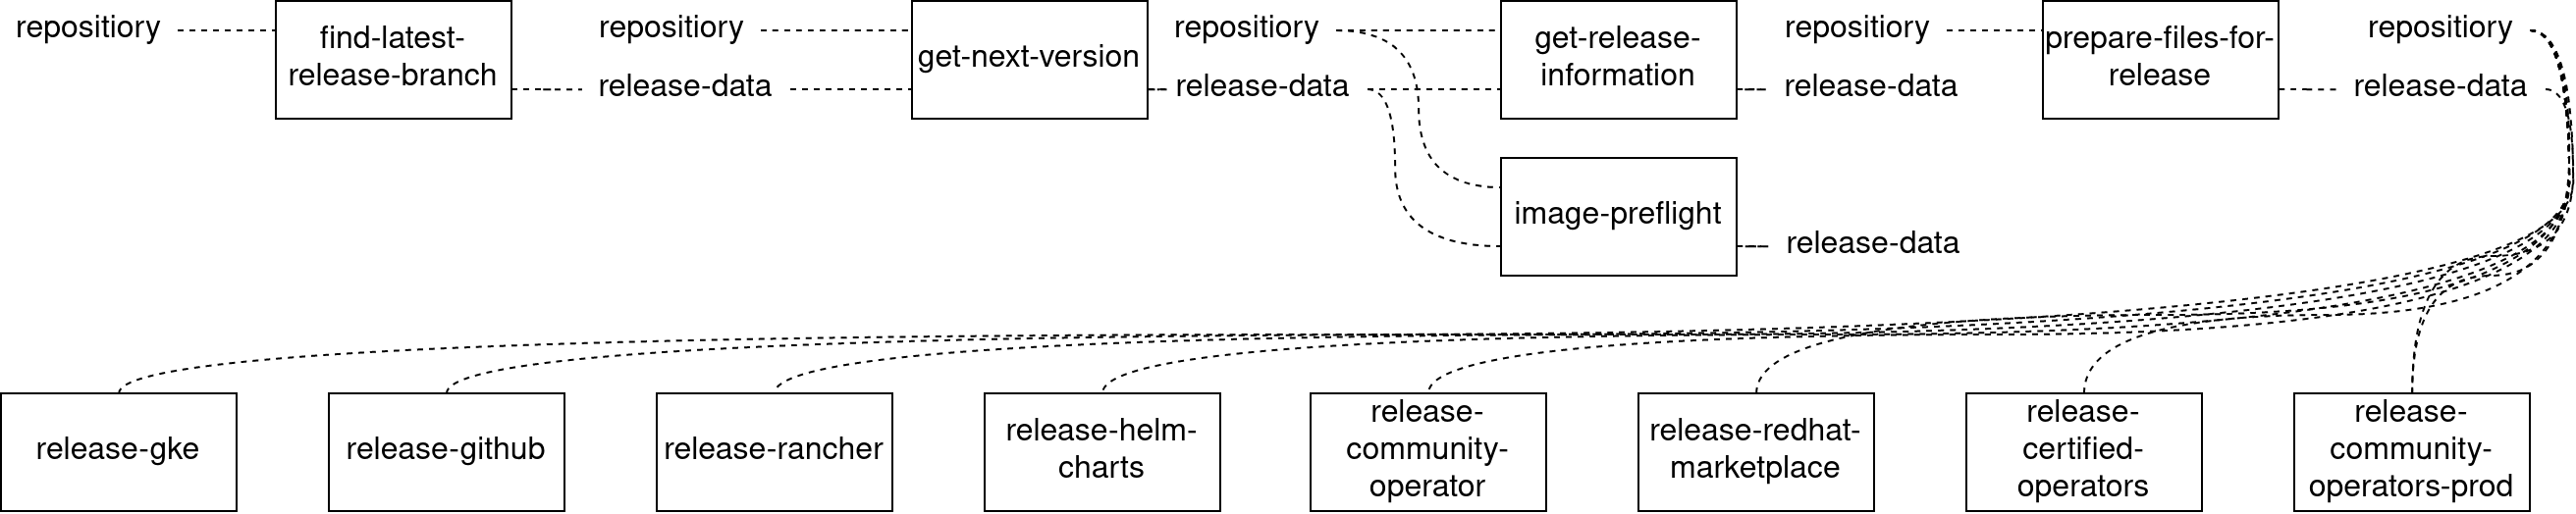
\includegraphics[width=\textwidth]{img/implementation/release-pipeline.drawio}
    \caption{Implemented release pipeline}
    \label{fig:implemented-release-pipeline}
\end{figure}

This section discusses the tasks implemented as part of the main release pipeline.
In figure~\ref{fig:implemented-release-pipeline} the final implementation of this pipeline part is depicted.
The boxes contain the names of the tasks, while the freestanding text depicts the resources they either consume or produce.
Most of them consume the DTO's repository and the release-data generated by the previous task.
They then generate a new version of the release-data, amended with the data generated by the tasks.

\subsection{Finding the latest release branch}\label{subsec:finding-the-latest-release-branch}

The purpose of this task is to automatically find the branch to operate on, since pipeline is designed to generate releases for the next version of the operator.
Since the script already parses version information, the branch names which are used by other tasks to generate CSV files and Helm charts on are also generated.
Furthermore, it filters any branches which are not used for releases, to avoid generating wrong files.

This task finds the latest release branch using the branches from the GitHub repository of the DTO.
First, the repository is cloned.
Then, the command \\
\verb%git branch -a | grep "${RELEASE_BRANCH_PREFIX}" > ../branches% \\
is used to query all branches, filter the ones with the appropriate prefix and write their names into a file.
The prefix which is used for filtering the names can be configured with the \verb|release_branch_prefix| parameter.
Afterwards a python script, which takes the following parameters, is called.

\begin{table}
    \centering
    \caption{Parameters for the python script finding a release branch}
    \label{tab:py-finding-the-release-branch}
    \begin{tabular}{l|l}
        Parameter & Expected value \\
        \hline
        \verb|--branch-list| & The path to the file containing the filtered branch names \\
        \verb|--release-prefix| & The prefix used to mark release branches. \\
        & It can be configured using the \verb|release_branch_prefix| parameter. \\
        \verb|--csv-prefix| & A prefix for a branch on which the CSV files are generated. \\
        & It can be configured using the \verb|csv_branch_prefix| parameter. \\
        \verb|--helm-prefix| & A prefix for a branch on which the Helm charts are generated. \\
        & It can be configured using the \verb|helm_branch_prefix| parameter. \\
        \verb|--output| & The path to which the results are written. \\
    \end{tabular}
\end{table}

This python script, using the parameters shown in table \ref{tab:py-finding-the-release-branch}, reads through the list of branches, tries to find a version for each one and then compares the versions found.
It does so, by first removing the strings \verb| {release-prefix}-v | and \verb| {release-prefix}- | from the name.
The resulting name is then split by a dot, i.e., \verb| . |, because it assumes the usage of a semantic versioning scheme.
Since the branches usually contain two version numbers, the major and minor version, the resulting array is extended with \verb| .0 | until is length is two.
These steps are necessary to obtain a normalized array for further processing.

The normalized arrays of two branches are then compared to each other.
If an array has a length greater than two, it is not in the expected form for release branches and is discarded.
If an element of the array cannot be parsed to an integer value, it is not in the semver format and is discarded.
If the elements of both arrays can be parsed, they are compared to each other.
If one element is larger then the element with the same index in the other array, it is considered as the later version.

Examples:
\begin{itemize}
    \item The branch \verb| release-v0.2 | is considered lower than \verb| release-v0.3 |
    \item The branch \verb| release-0.2 |  is considered lower than \verb| release-v0.2.1 |
    \item The branch \verb| release-1.3 | is considered later than \verb| release-0.5 |
    \item The branch \verb| release-2.0.0 | is considered invalid since is has too many version numbers. \\ Therefore any other branch ''wins'' the comparison.
    \item The branch \verb| release-vA.B | is considered invalid since \verb| A | cannot be parsed as an integer. \\ Therefore any other branch ''wins'' the comparison.
    \item The branch \verb| release-1 | is considered later than \verb| release-0.9 |. \\ The former version is appended with zeros. \\ The actual comparison would be \verb| 1.0 | against \verb| 0.9 |.
\end{itemize}

After the latest release branch is found, the version from it is also used to generate the CSV and Helm chart branches.
The resulting branches are \verb`{csv-prefix}-{version}` and \verb`{helm-prefix}-{version}`.
The following string is then written to the \verb`{output}` path.

\begin{verbatim}
{
    "branch": "<latest release branch>",
    "version": "<version of the latest release branch>",
    "csv_branch": "<generated CSV branch name>",
    "helm_branch" "<generated Helm branch name>"
}
\end{verbatim}


\pagebreak
\subsection{Get next version}\label{subsec:get-next-version}

This task uses the version found in the previous task from section \ref{subsec:finding-the-latest-release-branch} to infer the next patch version.
It does so by first querying all GitHub releases.
Then, they are filtered by the version found in the previous task.
For example, if releases exist on GitHub for the version 0.2.0, 0.2.1, 0.3.0, 0.3.1, and 0.4.0, and the release branch has a 0.4 postfix, only the 0.4.0 release is considered.
After the releases have been filtered, their titles, consisting of the version, are compared, similar to the comparison done between branches in the previous task.
From the latest release, the patch version is increase by one, and then saved in the JSON result as the new version.

The purpose of this task is to find the next version number.
Since the release branch names do not contain a patch number, it has to be inferred.
If releases exist for a \verb|major.minor| combination, the patch version of the latest release can just be bumped.
Otherwise, the patch version is \verb|0|.

The querying, filtering and comparison of releases is done again using a python script.
For the script to work, a GitHub token and the target repository have to be supplied as well as the branch version.
Therefore, the script takes the arguments shown in table \ref{tab:py-finding-the-next-version}.

\begin{table}[H]
    \centering
    \caption{Parameters for the python script finding the next version}
    \label{tab:py-finding-the-next-version}
    \begin{tabular}{p{0.3\linewidth}|p{0.6\linewidth}}
        Parameter & Expected value \\
        \hline
        \verb|--version| & Expects the version found by parsing the release branches from the previous task.  \\
        \verb|--token| &  A personal access token for GitHub.
            It should have the following scopes \verb|admin:org, delete_repo, repo, workflow|.
            The same token can be used by multiple tasks if these scopes are set. \\
        \verb|--operator-repository| & The target repository from which the releases are queried. \\
        \verb|--output| & The path to which the calculated version is written. \\
    \end{tabular}
\end{table}

\pagebreak

After parsing the arguments, the script creates an instance of \verb|GitHubApi|.
This class implements the Representational State Transfer (REST) requests provided by the GitHub API.
From this instance, the \verb|find_releases| function is called.
The URL used for the request is built by a static prefix \verb|https://api.github.com/repos/|, followed by the target repository name.
A \verb|/releases| prefix is then added as well to specifically target releases.
E.g., if the repository's name is \verb|Dynatrace/dynatrace-operator| the resulting URL is \verb|https://api.github.com/repos/Dynatrace/dynatrace-operator/releases|.
The header for this request contains the fields shown in table \ref{tab:http-header}.

\begin{table}[H]
    \centering
    \caption{HTTP Header}
    \label{tab:http-header}
    \begin{tabular}{p{0.3\linewidth}|p{0.6\linewidth}}
        Header field name & Value \\
        \hline
        Accept & \verb|application/vnd.github.v3+json| \\
        Authorization & \verb|token <GitHub Token>| \\
        Content-Type & \verb|application/json| \\
    \end{tabular}
\end{table}

If the request does not succeed, an error is returned.
Otherwise, the body of the request contains all releases for the target repository as a JSON-array.
The body is then converted into an array of instance of type \verb|GitHubRelease|.
This class does not implement specific functions, but is only used to hold the data from the request.

All found releases are then filtered.
Releases are discarded if:
\begin{itemize}
    \item They are a draft
    \item They do not contain the release branch version
    \item They are a sub-release of some kind.
        I.e., if they do not contain the character ``-''
\end{itemize}

Every release that was not discarded is then compared against the other, not discarded, releases.
The latest one is then taken.
From this release, the version is parsed from the tag and the patch version is increased by one.
If there exists no release for the current major-minor version combination, the resulting version defaults to \verb|major.minor.0|.
The result is then written to the output path.
Finally, the task finishes after updating the resulting JSON-data with the next version.


\textbf{Get release information}

This task's main purpose is to get the generated changelogs from the GitHub API.
To do so, the GitHub API expects the branch hash to know for which commit to generate changelogs for.
All additional information is then also added to the resulting release data.

This task is used to generate a changelog and collect metadata.
First, the branches SHA-hash is determined, by cloning the target repository and switching to the release branch, that was determined by the task for finding the latest release branch.
The bash command \verb|git rev-parse "${branch}"| then returns the hash value, which is used later.

Then, the prefix for the Google Container Registry (GCR)\footnote{https://cloud.google.com/container-registry} is determined.
The task uses the GKE service account, that is retrieved from a vault secret, to query the project name.
By adding the prefix \verb|gcr.io/| and replacing colons with forward slashes, the registry for the image, which is built and uploaded in a later task, can be determined.
The project name depends on the set marketplace value.
It can be configured by changing the \verb|gcp_marketplace| parameter.
Usually, these steps result in the prefix \verb|gcr.io/{gcp_marketplace}|.

After the project name and the branch hash are determined, a python script is called.
This script takes the parameters shown in Table~\ref{tab:params-to-generate-release-information}.

\begin{table}[h]
    \centering
    \caption{Parameters to generate release information.}
    \label{tab:params-to-generate-release-information}
    \begin{tabular}{p{0.3\linewidth}|p{0.6\linewidth}}
        Parameter & Expected value \\
        \hline
        \verb|--release-data| & The path to the release data currently compiled by previous tasks.  \\
        \verb|--branch-sha| & The release branches hash value as determined before. \\
        \verb|--github-token| & A personal access token for GitHub.
            It should have the following scopes \verb|admin:org|, \verb|delete_repo|, \verb|repo|, \verb|workflow|.
            The same token can be used by multiple tasks if these scopes are set \\
        \verb|--operator-repository| & The target repository from which the releases are queried \\
        \verb|--gke-registry| & The name of the GCR registry for the GKE release step later on. \\
        \verb|--gke-app-name| & The name under which the DTO is released. \\
    \end{tabular}
\end{table}

This script then proceeds to compile the given data, excluding the token and repository, together into a dictionary.
The descriptions for the GitHub and Helm releases are also added.
It then uses the token to request a changelog for the given repository from the GitHub API.
Similarly to how the task to get the next version requests releases, this script calls the \url{https://api.github.com/repos/<operator_repository>/releases/generate-notes} endpoint.
The generated changelog is then also appended to the resulting release data.
This task should then output the following JSON document.

\begin{verbatim}
{
    "branch": "<release-branch>",
    "version": "<next version to be release>",
    "csv_branch": "<branch on which to generate CSV files>",
    "helm_branch": "<branch on which to generate the Helm release>",
    "tag": "<the tag for the GitHub release>",
    "sha": "<hash of the release branch>",
    "release": {
        "changelog": "<Changelog generated by the GitHub API>",
        "description": "<Hardcoded description for the GitHub release>",
        "helm-chart-description": "<Hardcoded description for the Helm release>"
    },
    "gcr": {
        "registry": "<GCR registry as determined before>",
        "app-name": "dynatrace-operator",
        "version": "<next version to be release>",
        "image": "<GCR image name for the operator release>"
    }
}
\end{verbatim}


\subsection{Image preflight}\label{subsec:image-preflight}

The purpose of this task is to automatically check if necessary images are available on all registries.
Furthermore, it finds the digests of the DockerHub and RHCC images, so the images in the CSVs can be digest-pinned.

This task is used to check whether all images necessary for this release are available.
It needs the Docker config defined as a vault secret to have access to the necessary registries.
Furthermore, it uses a Docker in Docker image to try and pull the images.
Finally, it parses the digests of the images and adds them to the release information.

First \verb| jq | is installed to read the release data, since \verb| jq | is not installed by default on the Docker in Docker image.
Then, the Docker config provided is written to \verb| ~/.docker/config.json | to make it available to Docker.
The command \verb| source /docker-lib.sh | imports all functions made available by the Docker in Docker image.
One of the functions is \verb| start_docker |, which is then called to start the Docker daemon.

Then the availability of the following images is checked.
* \verb| registry.connect.redhat.com/dynatrace/dynatrace-operator:v${version} |
* \verb| gcr.io/${GCE_MARKETPLACE}/dynatrace-operator:${version} |
* \verb| docker.io/dynatrace/dynatrace-operator:v${version} |

Where \verb| version | is read from the release data using jq.
\verb| ${GCE_MARKETPLACE} | is defined by the \verb| gcp_marketplace | parameter.
If any of those image cannot be pulled, the task fails.

The digest is then parsed for each image.
From the \verb| docker pull | command, for the DockerHub and RHCC image, the response is taken.
Since the digest can be found in the response, it is parsed from there using \verb| grep "Digest:" | to find the line.
Then, using shell expansion, the ''Digest: '' prefix is removed with \verb| ${digest#"Digest: "} |.
This functionality is used twice and therefore put into a function called \verb| parse_digest | which takes the response from the pull command as its parameter.


\textbf{Prepare files for release}

The task generates the CSV bundles for Openshift and Kubernetes OLM systems.
Since most files and information is available, minor changes like setting version properties are also done.

This task is used to generate the CSV bundles for the OLM releases as well as setting minor details in other files.
To do so, it first needs to install the Operator SDK.
The version to download can be configured with the \verb|operator_sdk_version| parameter.
If the parameter is not set, the latest version available is downloaded.

\pagebreak

Then the release branch is checked out of the target repository.
From this branch, the CSV branch is created.
In order to get a clean branch, it is first deleted if it exists and the deletion is force pushed afterwards.
Force deleting the branch will close open pull requests that are based on this branch.

Afterwards, the following changes are made. \\
In \verb|<repository>/config/helm/chart/default/Chart.yaml|:
\begin{itemize}
    \item The \verb| version | property is set to the version which is going to be released
    \item The \verb| appVersion | property is set to the version which is going to be released
    \item Setting this property is done using a library, which does not preserve comments.
    Therefore, the license text is re-added to the top afterwards
\end{itemize}

In \verb|<repository>/config/helm/schema.yaml|
\begin{itemize}
    \item The \verb| x-google-marketplace.publishedVersion | property is set to the version which is going to be released
    \item The \verb| x-google-marketplace.publishedVersionMetadata.releaseNote | property is set to the generated changelog
    \item Again, the license text is re-added afterwards
\end{itemize}

In \verb|dynatrace-operator/config/helm/chart/default/templates/application.yaml|
\begin{itemize}
    \item The \verb|version| property is set to the version which is going to be released
    \item This file is a Helm template, which has some extended notations compared to a normal YAML file.
        Therefore, the same library used before cannot be used here to set this property.
    \item In order to mitigate this problem, the replacement is done using \verb|sed| and the license text does not need to be re-added.
\end{itemize}

Then, the CSV bundles are generated.
Once for Kubernetes, another time for Openshift.
A target of the Makefile included in the dynatrace-operator repository is used to generate these files.
The following parameters are set to make sure the image is correctly replaced for each platform.

For Kubernetes, the following parameters are set.

\begin{verbatim}
IMG="docker.io/dynatrace/dynatrace-operator:v${version}"
MASTER_IMAGE="docker.io/dynatrace/dynatrace-operator:v${version}"
BRANCH_IMAGE="docker.io/dynatrace/dynatrace-operator:v${version}"
OLM_IMAGE="docker.io/dynatrace/dynatrace-operator:v${version}"
\end{verbatim}

For Openshift, the following parameters are set.

\begin{verbatim}
IMG="registry.connect.redhat.com/dynatrace/dynatrace-operator:v${version}"
BRANCH_IMAGE="registry.connect.redhat.com/dynatrace/dynatrace-operator:v${version}"
MASTER_IMAGE="registry.connect.redhat.com/dynatrace/dynatrace-operator:v${version}"
OLM_IMAGE="registry.connect.redhat.com/dynatrace/dynatrace-operator:v${version}"
\end{verbatim}

Finally, the generated CSV files are finalized by a python script.
This script main purpose is to set the correct date for the \verb|metadata/annotations/createdAt| property in the main CSV files.
It also sets the \verb|spec/replaces| field to the version of the last GitHub release, however, this value is only used as a fallback.
This property is later overwritten to depend on the release CSV files instead of the released GitHub versions.

After all changes were made, they are pushed to the CSV branch.
Finally, a pull request from the CSV branch to the release branch is created.



\textbf{Release GKE}

This job consists of multiple tasks.
Their goal is to build and push the deployer image for GCM, prepare a GKE cluster, install the deployer image on it and check if a basic Operator deployment succeeds.

\textit{Building and pushing a deployer image}

The purpose of this task is to build a deployer image and publish it to GCR.
This task builds the Dockerfile at \verb|<repository>/config/helm/| and pushes the resulting image to GCR as the deployer image.

\textit{Preparing a cluster}

The purpose of this task is to prepare a GKE cluster for the deployment of a deployer image.
This includes cleaning any leftover resources created by a previous DTO deployment and applying the GKE Application CRD.
This task prepares a GKE cluster to be able to deploy the previously built deployer image.
First, the kube-config is read from the vault secret, which is set by the task of section~\ref{subsubsec:fetch-kubeconfig}.
Therefore, for this task, and by extension this job, to succeed, a GKE cluster must be running.
A GKE cluster can be created with the task of section~\ref{subsec:create-release-gke-infrastructure}.

After the kube-config is read and written to \verb|\${HOME}/.kube/config|, the GCPs application CRD is applied from \url{https://raw.githubusercontent.com/GoogleCloudPlatform/marketplace-k8s-app-tools/master/crd/app-crd.yaml}.
This CRD is needed so GCP applications can be deployed.
If the \verb|dynatrace| namespace or the DynaKube CRD exist on the cluster, they are deleted to ensure a clean state.
Afterwards, the namespace is created and the DynaKube CRD is applied again.

\textit{Installing the deployer image}

The purpose of this task is to deploy the deployer image on a prepared GKE cluster.
The deployment is then monitored by the next task.
This task uses Google's \verb|mpdev| tool to deploy the deployer image onto the cluster mentioned above.
Since it also uses a Docker in Docker image, it first installs \verb|jq| to read the image name from the release data.
It then installs the \verb|mpdev| tool and prepares the kube-config file as well as the GKE service account.

The \verb|mpdev| tool can take parameters which are passed to the custom resource of the DTO.
In order to check a simple deployment, the following properties are given to the tool in the JSON format.

\begin{verbatim}
{
    "name": "dynatrace-operator",
    "namespace": "dynatrace",
    "apiUrl": "<a valid API url>",
    "apiToken": "<a valid api token for the given API>",
    "paasToken": "<a valid paas token for the given API>"
}
\end{verbatim}

The API URL, the API token, as well as the PAAS token, are defined as vault secrets.
After executing a command, \verb|./mpdev install|, with the parameters \verb|--deployer="${image}"| and \verb|--parameters="${parameters}|, \verb|mpdev| deploys the deployer image with the parameters from above.

\textit{Sanity checking the deployer deployment}

This tasks purpose is to make a quick test whether the deployer image can deploy the DTO successfully or not.
This task checks the deployment job, that the \verb|mpdev| tool creates, for its success.
To do so, it again sets up the kube-config.
Afterwards, the condition type of the job \verb|job/dynatrace-operator-deployer| is monitored.

\begin{itemize}
    \item If it does not reach the state \verb|Complete| after five minutes, the task fails.
    \item If the job reaches this state, the \verb|.status.succeeded| flag is checked.
    \item If the job did not succeed, the task fails.
    \item If the job succeeded, the pod's states are checked by a Python script.
    \item If the pod's states are \verb|Terminated| and the reason is \verb|Error|, the task fails.
    \item If the job completes successfully and all DTO pods are running afterwards, the task succeeds and the deployer image can be assumed to work.
\end{itemize}


\subsection{Release GitHub}\label{subsec:release-github}

This task creates a GitHub release for the manifest files and the DTO Helm charts.
It first checks out the release branch of the DTO repository and creates a new branch with the value of \verb|helm_branch| in the release data.
If this branch already exists it is force deleted, to also close and remove any open pull requests.
This way, a consistent state is ensured.
Then, the Helm package is generated.

First, the GPG keyring, which is defined as a vault secret, is set up.
\begin{itemize}
    \item A directory is created at \verb|~/.gnupg/|.
    \item The secret for \verb|pubring| is decoded and written to \verb|~/.gnupg/pubring.gpg|.
    \item The secret for \verb|secring| is decoded and written to \verb|~/.gnupg/secring.gpg|.
    \item The secret for the password to the keyring is written to \verb|~/.gnupg/password|.
\end{itemize}

The folder \verb|~/.gnupg/| is then given \verb|700| as permission bits.
The created files get \verb|600| as permission bits.
By issuing the command \verb|gpg --list-secret-keys|, the existence of the keyring can be confirmed.

Then, the following command is issued.

\begin{verbatim}
helm package \
    "./dynatrace-operator/config/helm/chart/default/" \
    -d "./dynatrace-operator/config/helm/repos/stable/" \
    --app-version "${version}" \
    --version "${version}" \
    --sign \
    --key "Dynatrace LLC" \
    --keyring ~/.gnupg/secring.gpg \
    --passphrase-file ~/.gnupg/password
\end{verbatim}

The first argument points to the Helm charts which are packaged.
The \verb|-d| option defines where the new package is written to.
With the \verb|--sign| option, the GPG keyring is used to sign the package, while the \verb|--keyring| option defines which keyring to use.
\verb|--key| sets which of the secrets in the keyring to use and \verb|--passphrase-file| defines where to find the password the secret expects.

After the package is generated, the Helm index \verb|index.yaml|, which lists available packages, is copied to \verb|index.yaml.previous|.
The importance of this file is explained later on.
Then, the index is regenerated with the following command.
The \verb|--url| parameter must point to the path where the \verb|index.yaml| will be available after the release.

\begin{verbatim}
helm repo index ./dynatrace-operator/config/helm/repos/stable/ \
--url "https://raw.githubusercontent.com/\${operator_repository}
        /master/config/helm/repos/stable"
\end{verbatim}

Then a python script prepares the Helm index.
Here the importance of the copy of the index becomes apparent.
Every entry of a version has a \verb|created| field which stores the date at which it was created.
If the index is regenerated, all those fields are updated with the current date.
An old version would then have the same creation date as the latest one.
Therefore, the correct dates from \verb|index.yaml.previous| are read and then reapplied to the new index using this python script.
Then, the manifests are generated for each platform, Kubernetes and Openshift.
Similar to generating the bundle, i.e., CSV, files, the following properties are added to the \verb|make manifest| command, to make sure the image is set correctly.

\textbf{Kubernetes}

\begin{verbatim}
IMG="docker.io/dynatrace/dynatrace-operator:v${version}"
BRANCH_IMAGE="docker.io/dynatrace/dynatrace-operator:v${version}"
MASTER_IMAGE="docker.io/dynatrace/dynatrace-operator:v${version}"
OLM_IMAGE="docker.io/dynatrace/dynatrace-operator:v${version}"
\end{verbatim}

\textbf{Openshift}

\begin{verbatim}
IMG="registry.connect.redhat.com/dynatrace/dynatrace-operator:v${version}"
BRANCH_IMAGE="registry.connect.redhat.com/dynatrace/dynatrace-operator:v${version}"
MASTER_IMAGE="registry.connect.redhat.com/dynatrace/dynatrace-operator:v${version}"
OLM_IMAGE="registry.connect.redhat.com/dynatrace/dynatrace-operator:v${version}"
\end{verbatim}

The generated Helm package, index and manifests are then added, committed and pushed to the repository.
A pull request is then created.

A python script then creates a draft release and uploads the artifacts to it.
For the script to work, a GitHub token and the target repository have to be supplied as well as the generated release data.
Therefore, the script takes the arguments shown in table \ref{tab:parameters-for-release-generation}.

\begin{table}[H]
    \centering
    \caption{Parameters for release generation}
    \label{tab:parameters-for-release-generation}
    \begin{tabular}{p{0.3\linewidth}|p{0.6\linewidth}}
        Parameter & Expected value \\
        \hline
        \verb|--release-data| & Expects the version found by parsing the release branches form the previous task. \\
        \verb|--token| & A personal access token for GitHub.
            It should have the following scopes \verb|admin:org, delete_repo, repo, workflow|.
            The same token can be used by multiple tasks if these scopes are set. \\
        \verb|--operator-repository| & The target repository from which the releases are queried \\
    \end{tabular}
\end{table}

After parsing the arguments, the script creates an instance of \verb|GitHubApi|.
This class implements some REST requests provided by the GitHub API.
From the \verb|GitHubApi| instance, the \verb|create_release| function is called.
This function takes an instance of \verb|GitHubRelease|.
\verb|GitHubRelease| bundles all information needed for a release.

The \verb|create_release| function then uses the release data to send a post request to GitHub's release endpoint.
The URL used for the request is built by a static prefix \url{https://api.github.com/repos/}, followed by the target repository name.
A \verb|/releases| postfix is then added as well to specifically target releases.
E.g., if the repository's name is \verb|Dynatrace/dynatrace-operator| the resulting URL is \url{https://api.github.com/repos/Dynatrace/dynatrace-operator/releases}.
The header for this request contains the fields described in table \ref{tab:header-fields-to-create-a-release-request}.

\begin{table}[H]
    \centering
    \caption{Header fields to create a release request}
    \label{tab:header-fields-to-create-a-release-request}
    \begin{tabular}{p{0.3\linewidth}|p{0.6\linewidth}}
        Header field name & Value \\
        \hline
        Accept & \verb|application/vnd.github.v3+json|  \\
        Authorization & \verb|token <GitHub Token>| \\
        Content-Type & \verb|application/json| \\
    \end{tabular}
\end{table}

The changelog for the GitHub release is left to be generated by GitHub.
If the request does not succeed and does not return a response with a 201 HTTP code, an error is printed and nothing is returned.
The response body of a successful request contains a URL to upload assets to, the \verb|upload_url|.
This upload URL is returned by the \verb|create_release| function.
The script then proceeds to upload the assets necessary for the release, which were previously generated.

In order to upload assets, the \verb|try_upload_asset| function of the \verb|GitHubApi| instance is used.
It uploads the assets to the \verb|upload_url| from before.
The header for the request contains similar fields to the ones of table \ref{tab:header-fields-to-create-a-release-request}.
The \verb|Content-Type| is usually changed to \verb|application/octet-stream| to signify the upload of a file.
If the upload fails, \verb|try_upload_asset| returns \verb|False| and prints the error message, otherwise it returns true \verb|True|.
If uploading an asset fails, the task fails.


\subsection{Release Rancher}\label{subsec:release-rancher}

This task releases the DTO helm chart to the Rancher repository for partner charts.
It first clones the DTO repository and then create a fork of Rancher's repository.
Forking is done by a python script that can be found at [/scripts/release/fork.py](../../scripts/release/fork.py).
This script takes the following arguments.

| Parameter               | Expected value                                                                                                                                                                         | Default          |
| ----------------------- | -------------------------------------------------------------------------------------------------------------------------------------------------------------------------------------- | ---------------- |
| `--token`               | A personal access token for GitHub. It should have the following scopes `admin:org, delete_repo, repo, workflow`. The same token can be used by multiple tasks if these scopes are set |                  |
| `--original-repository` | The original repository which should be forked                                                                                                                                         |                  |
| `--forked-repository`   | The name the forked repository should have                                                                                                                                             |                  |
| `--output-file`         | The path to which the metadata of the fork is written to                                                                                                                               | `fork-data.json` |
| `--retries`             | How often the scripts should retry requests should they fail                                                                                                                           | `10`             |
| `--retry-timeout`       | How long, in seconds, the script waits between request retries.                                                                                                                        | `5`              |

After parsing the arguments, an instance of `GitHubApi`, a class found in [/scripts/release/github/github_api.py](../../scripts/release/github/github_api.py), is created using `{forked-repository}` and `{token}`.
This class implements some REST requests GitHub's API provides.
First, the `exists` function is called, which returns `True` if the forked repository already exists.
To ensure a consistent environment, forked repositories are deleted if they already exist.
Therefore, if the `exist` function returns true, the fork is deleted by calling `delete_repository`, which returns `True` if the request succeeds or `False` if it doesnt.
Additionally, the response from the GitHub API is also returned.

If the forked repository does not exist or has successfully been deleted, it is recreated.
This is done by calling the `fork` function and passing `{original-repository}` as a parameters.
On a success, a check is made, if the forked repository has the expected name `{forked-repository}`.
If it does not, the repository is renamed by instantiating `GitHubApi` with the newly forked repository and calling the `rename` function.
The metadata of the forked repository is then written to `{output-file}`.

When the fork has been created, the task continues to clone it and check out a new branch `dynatrace-operator-v${version}`.
On this branch, a new directory for the version of the new release is created, committed and pushed.
Then, the contents of `{repository}/config/helm/chart/default/`, i.e., the DTO Helm charts, are copied to this new directory.
In the copy of the `Chart.yaml`, the icon property is then set to `file://../logo.png`, to reference the local file.
Finally, the changes are add, committed and pushed to the forked repository.

## Purpose

The purpose of this task is to execute all steps necessary to release the DTO Helm charts to Rancher.
This includes forking their repository and follow their guidelines.
A pull request or draft pull request is not done to avoid operating on a foreign repository with automatic tasks.


\subsection{Release community operators}\label{subsec:release-community-operators}

This task releases the CSV bundle for Kubernetes to the community operators repository.
Releasing the CSV files to this repository makes the DTO available on OperatorHub.
The purpose of this task is to execute all steps necessary to release the CSV bundle to OperatorHub.
This includes forking the repository and following the OperatorHub guidelines.
A pull request or draft pull request is not done to avoid operating on a foreign repository with automatic tasks.

It first clones the DTO repository and then creates a fork of the community operators repository using a Python script
This script takes the following arguments.

\begin{table}[H]
    \centering
    \caption{Parameters to clone and fork a repository}
    \label{tab:parameters-to-clone-and-fork-a-repository}
    \begin{tabular}{p{0.3\linewidth}|p{0.6\linewidth}}
        Parameter & Expected value \\
        \hline
        \verb|--token| & A personal access token for GitHub.
            It should have the following scopes \verb|admin:org, delete_repo, repo, workflow|.
            The same token can be used by multiple tasks if these scopes are set. \\
        \verb|--original-repository| & The original repository which should be forked. \\
        \verb|--forked-repository| & The name the forked repository should have. \\
        \verb|--output-file| & The path to which the metadata of the fork is written to. \\
        \verb|--retries| & How often the scripts should retry requests should they fail. \\
        \verb|--retry-timeout| & How long, in seconds, the script waits between request retries. \\
    \end{tabular}
\end{table}

After parsing the arguments, an instance of \verb|GitHubApi| is created using \verb|{forked-repository}| and \verb|{token}|.
This class implements some REST requests GitHub's API provides.
First, the \verb|exists| function is called, which returns \verb|True| if the forked repository already exists.
To ensure a consistent environment, forked repositories are deleted if they already exist.
Therefore, if the \verb|exist| function returns true, the fork is deleted by calling \verb|delete_repository|, which returns \verb|True| if the request succeeds or \verb|False| if it doesnt.
Additionally, the response from the GitHub API is also returned.

If the forked repository does not exist or has successfully been deleted, it is recreated.
This is done by calling the \verb|fork| function and passing \verb|{original-repository}| as a parameters.
On a success, a check is made, if the forked repository has the expected name \verb|{forked-repository}|.
If it does not, the repository is renamed by instantiating \verb|GitHubApi| with the newly forked repository and calling the \verb|rename| function.
The metadata of the forked repository is then written to \verb|{output-file}|.
In this forked repository, the following folders are created for the new version.

\begin{verbatim}
${fork_name}/operators/dynatrace-operator/${version}/manifests
${fork_name}/operators/dynatrace-operator/${version}/metadata
\end{verbatim}

The Dockerfile located at \verb|{repository}/config/olm/kubernetes/bundle-${version}.Dockerfile| is placed in the version's folder.
The previously mentioned folders, are then populated with the CSV bundles from \verb|{repository}/config/olm/kubernetes/${version}/manifests| and \verb|{repository}/config/olm/kubernetes/${version}/metadata| respectively.
Finally, the changes are added, committed and pushed to the forked repository.


# release-redhat-marketplace

This task releases the CSV bundle for Openshift to the RedHat marketplace repository.
Releasing the CSV files to this repository makes the DTO available on the RedHat Marketplace for Operators.

It first clones the DTO repository and then creates a fork of the RedHat marketplace repository.
Forking is done by a python script that can be found at [/scripts/release/fork.py](../../scripts/release/fork.py).
This script takes the following arguments.

| Parameter               | Expected value                                                                                                                                                                         | Default          |
| ----------------------- | -------------------------------------------------------------------------------------------------------------------------------------------------------------------------------------- | ---------------- |
| `--token`               | A personal access token for GitHub. It should have the following scopes `admin:org, delete_repo, repo, workflow`. The same token can be used by multiple tasks if these scopes are set |                  |
| `--original-repository` | The original repository which should be forked                                                                                                                                         |                  |
| `--forked-repository`   | The name the forked repository should have                                                                                                                                             |                  |
| `--output-file`         | The path to which the metadata of the fork is written to                                                                                                                               | `fork-data.json` |
| `--retries`             | How often the scripts should retry requests should they fail                                                                                                                           | `10`             |
| `--retry-timeout`       | How long, in seconds, the script waits between request retries.                                                                                                                        | `5`              |

After parsing the arguments, an instance of `GitHubApi`, a class found in [/scripts/release/github/github_api.py](../../scripts/release/github/github_api.py), is created using `{forked-repository}` and `{token}`.
This class implements some REST requests GitHub's API provides.
First, the `exists` function is called, which returns `True` if the forked repository already exists.
To ensure a consistent environment, forked repositories are deleted if they already exist.
Therefore, if the `exist` function returns true, the fork is deleted by calling `delete_repository`, which returns `True` if the request succeeds or `False` if it doesnt.
Additionally, the response from the GitHub API is also returned.

If the forked repository does not exist or has successfully been deleted, it is recreated.
This is done by calling the `fork` function and passing `{original-repository}` as a parameters.
On a success, a check is made, if the forked repository has the expected name `{forked-repository}`.
If it does not, the repository is renamed by instantiating `GitHubApi` with the newly forked repository and calling the `rename` function.
The metadata of the forked repository is then written to `{output-file}`.

In this forked repository, first, the latest released version is determined.
A python script, located at [/scripts/release/directory_version.py](../../scripts/release/directory_version.py), iterates over the directories in the `dynatrace-operator-rhmp` folder.
The directories are named after the released version, i.e., `0.2.2`, `0.3.0`, etc.
The latest version is then saved in a variable `last_version`.
If no version exist, it defaults to an empty string.

Afterwards, a new folder for the version to be released is created.
The folders, `${fork_name}/operators/dynatrace-operator-rhmp/${version}/manifests` and `${fork_name}/operators/dynatrace-operator-rhmp/${version}/metadata` are then populated with the CSV bundles from `{repository}/config/olm/openshift/${version}/manifests` and `{repository}/config/olm/openshift/${version}/metadata` respectively.
In the CSV file of the version to be released, the `replaces` property is then updated, if `last_version` is not empty.
If the variable is empty, the property is removed.
Setting this property allows Openshift to correctly update the DTO.

Then, annotations mentioning the string `dynatrace-operator` are changed to read `dynatrace-operator-rhmp` and the CSV file is renamed from `dynatrace-operator.clusterserviceversion.yaml` to `dynatrace-operator-rhmp.clusterserviceversion.yaml`.
This is necessary to reflect the different directory name RedHat has given it's Marketplace releases.
Finally, the changes are added, committed and pushed to the forked repository.

## Purpose

The purpose of this task is to execute all steps necessary to release the CSV bundle to the RedHat Marketplace for Operators.
This includes forking the repository and following the RedHat Marketplace guidelines.
A pull request or draft pull request is not done to avoid operating on a foreign repository with automatic tasks.

## Configuration options

The parameters can be changed in the [params-dev](../../params-dev.yaml) or [params-prod](../../params-prod.yaml) files.
The following parameters can be used to configure this task.

| Parameter                            | Effect                                                                                               | Production default                                        | Development default                                       |
| ------------------------------------ | ---------------------------------------------------------------------------------------------------- | --------------------------------------------------------- | --------------------------------------------------------- |
| `redhat_marketplace_repository`      | Defines the repository that should be forked. I.e., defines the value of `{original-repository}`     | `redhat-openshift-ecosystem/redhat-marketplace-operators` | `redhat-openshift-ecosystem/redhat-marketplace-operators` |
| `redhat_marketplace_repository_fork` | Defines the name the forked repository should have. I.e., defines the value of `{forked-repository}` | `dt-team-kubernetes/redhat-marketplace-operators`         | `dt-team-kubernetes/redhat-marketplace-operators`         |

## Common error cases

### The fork is not created properly

1. Check if the GitHub token is set correctly. It must not be expired and have the necessary scopes.
2. Check if the correct `redhat_marketplace_repository` is targeted.
3. Check if the correct fork, i.e. `redhat_marketplace_repository_fork`, is targeted

### The forked repository could not be found

1. Check that the name of the fork, i.e. `redhat_marketplace_repository_fork`, is set correctly.
2. Sometimes, when a fork is created by the GitHub API, the original name is suffixed by a counter, if the fork already existed on the target account.
   The python script that forks the repository should take care of renaming it, but if it fails to do so, the task may not continue successfully.

### The RedHat's CI pipeline fails

1. Close and re-open the pull request. 
   Sometimes their CI pipeline just fails without reason.
2. Check that the CSV files are correctly generated.
   Try to install them to a local Openshift cluster and deploy them manually.
   Make sure the Operator can deploy successfully with this install method.
3. Contact RedHat support.


\textbf{Release certified operators}

This task releases the CSV bundle for Openshift to the RedHat certified operators repository.
Releasing the CSV files to this repository makes the DTO available on the RedHat Catalog for certified Operators.

The purpose of this task is to execute all steps necessary to release the CSV bundle to the RedHat Catalog for Certified Operators.
This includes forking the repository and following the RedHat Catalog guidelines.
A pull request or draft pull request is not done to avoid operating on a foreign repository with automatic tasks.

It first clones the DTO repository and then creates a fork of the RedHat certified operators repository.
Forking is done by a python script that takes the arguments seen Table~\ref{tab:parameters-to-fork-the-certified-operators-repository}.

\begin{table}[H]
    \centering
    \caption{Parameters to fork the certified operators repository.}
    \label{tab:parameters-to-fork-the-certified-operators-repository}
    \begin{tabular}{|p{0.3\linewidth}|p{0.6\linewidth}}
        Parameter & Expected value \\
        \hline
        \verb|--token| & A personal access token for GitHub.
            It should have the following scopes \verb|admin:org|, \verb|delete_repo|, \verb|repo|, \verb|workflow|.
            The same token can be used by multiple tasks if these scopes are set. \\
        \verb|--original-repository| & The original repository which should be forked. \\
        \verb|--forked-repository| & The name the forked repository should have. \\
        \verb|--output-file| & The path to which the metadata of the fork is written to. \\
        \verb|--retries| & How often the scripts should retry requests should they fail. \\
        \verb|--retry-timeout| & How long, in seconds, the script waits between request retries. \\
    \end{tabular}
\end{table}

After parsing the arguments, an instance of \verb|GitHubApi| is created using \verb|{token}| and \verb|{forked-repository}|.
This class implements some REST requests GitHub's API provides.
First, the \verb|exists| function is called, which returns \verb|True| if the forked repository already exists.
To ensure a consistent environment, forked repositories are deleted if they already exist.
Therefore, if the \verb|exist| function returns true, the fork is deleted by calling \verb|delete_repository|, which returns \verb|True| if the request succeeds or \verb|False| if it doesn't.
Additionally, the response from the GitHub API is also returned.

\pagebreak

If the forked repository does not exist or has successfully been deleted, it is recreated.
This is done by calling the \verb|fork| function and passing \verb|{original-repository}| as a parameters.
On a success, a check is made, if the forked repository has the expected name \verb|{forked-repository}|.
If it does not, the repository is renamed by instantiating \verb|GitHubApi| with the newly forked repository and calling the \verb|rename| function.
The metadata of the forked repository is then written to \verb|{output-file}|.

In this forked repository, first, the latest released version is determined.
A python script iterates over the directories in the \verb|dynatrace-operator| folder.
The directories are named after the released version, i.e., \verb|0.2.2|, \verb|0.3.0|, etc.
The latest version is then saved in a variable \verb|last_version|.
If no version exist, it defaults to an empty string.

Afterwards, a new folder for the version to be released is created.
The folders for the manifests and the metadata are then populated with the generated CSV bundles.
In the CSV file of the version to be released, the \verb|replaces| property is then updated, if \verb|last_version| is not empty.
If the variable is empty, the property is removed.
Setting this property allows Openshift to correctly update the DTO.
Finally, the changes are added, committed and pushed to the forked repository.


\textbf{Release community operators prod}

This task releases the CSV bundle for Kubernetes to the community-operators-prod repository.
Releasing the CSV files to this repository makes the DTO available on the embedded OperatorHub in OpenShift and OKD.
The purpose of this task is to execute all steps necessary to release the CSV bundle to the embedded OperatorHub in OpenShift and OKD.
This includes forking the repository and following the OperatorHub guidelines.
A pull request or draft pull request is not done to avoid operating on a foreign repository with automatic tasks.

It first clones the DTO repository and then creates a fork of the community-operators-prod repository.
Forking is done by a python script that takes the arguments shown in Table~\ref{tab:parameters-to-fork-the-community-operators-prod-repository}.

\begin{table}[h]
    \centering
    \caption{Parameters to fork the community-operators-prod repository.}
    \label{tab:parameters-to-fork-the-community-operators-prod-repository}
    \begin{tabular}{p{0.3\linewidth}|p{0.6\linewidth}}
        Parameter & Expected value \\
        \hline
        \verb|--token| & A personal access token for GitHub.
            It should have the following scopes \verb|admin:org|, \verb|delete_repo|, \verb|repo|, \verb|workflow|.
            The same token can be used by multiple tasks if these scopes are set. \\
        \verb|--original-repository| & The original repository which should be forked. \\
        \verb|--forked-repository| & The name the forked repository should have. \\
        \verb|--output-file| & The path to which the metadata of the fork is written to. \\
        \verb|--retries| & How often the scripts should retry requests should they fail. \\
        \verb|--retry-timeout| & How long, in seconds, the script waits between request retries. \\
    \end{tabular}
\end{table}

After parsing the arguments, an instance of \verb|GitHubApi| is created using \verb|{token}| and \verb|{forked-repository}|.
This class implements some REST requests GitHub's API provides.
First, the \verb|exists| function is called, which returns \verb|True| if the forked repository already exists.
To ensure a consistent environment, forked repositories are deleted if they already exist.
Therefore, if the \verb|exist| function returns true, the fork is deleted by calling \verb|delete_repository|, which returns \verb|True| if the request succeeds or \verb|False| if it doesn't.
Additionally, the response from the GitHub API is also returned.

If the forked repository does not exist or has successfully been deleted, it is recreated.
This is done by calling the \verb|fork| function and passing \verb|{original-repository}| as a parameters.
On a success, a check is made, if the forked repository has the expected name \verb|{forked-repository}|.
If it does not, the repository is renamed by instantiating \verb|GitHubApi| with the newly forked repository and calling the \verb|rename| function.
The metadata of the forked repository is then written to \verb|{output-file}|.

In this forked repository, the folder \verb|version| folder is created inside the folder designated for the DTO for the new version.
The bundle's Dockerfile is placed in the version's folder.
The previously mentioned folder is then also populated with the generated CSV bundles.
Finally, the changes are added, committed and pushed to the forked repository.

